\documentclass{article}
% translate with >> pdflatex -shell-escape <file>

% This file is an extract of the PGFPLOTS manual, copyright by Christian Feuersaenger.
% 
% Feel free to use it as long as you cite the pgfplots manual properly.
%
% See
%   http://pgfplots.sourceforge.net/pgfplots.pdf
% for the complete manual.
%
% Any required input files (for <plot table> or <plot file> or the table package) can be downloaded
% at
% http://www.ctan.org/tex-archive/graphics/pgf/contrib/pgfplots/doc/latex/
% and
% http://www.ctan.org/tex-archive/graphics/pgf/contrib/pgfplots/doc/latex/plotdata/

\usepackage{pgfplots}
\pgfplotsset{compat=newest}

\pagestyle{empty}

\begin{document}
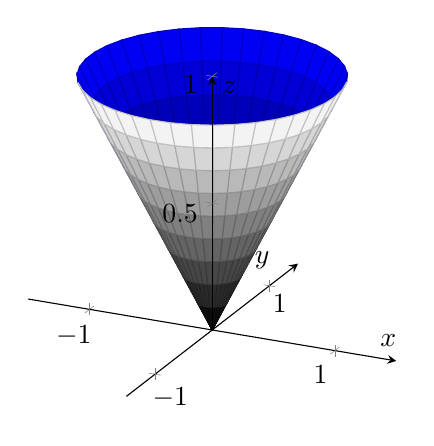
\begin{tikzpicture}
\begin{axis}[
  axis lines=center,
  axis on top,
  xlabel={$x$}, ylabel={$y$}, zlabel={$z$},
  domain=0:1,
  y domain=0:2*pi,
  xmin=-1.5, xmax=1.5,
  ymin=-1.5, ymax=1.5, zmin=0.0,
  mesh/interior colormap=
  	{blueblack}{color=(black) color=(blue)},
  colormap/blackwhite, 
  samples=10,
  samples y=40,
  z buffer=sort,
 ]
  \addplot3[surf] 
  	({x*cos(deg(y))},{x*sin(deg(y))},{x});
\end{axis}
\end{tikzpicture}
\end{document}
